\chapter{Разработка и экспериментальное внедрение системы радиочастотной идентификации}\label{ch:ch5}
Ключевая проблема, возникающая при построении системы радиочастотной идентификации транспортных средств "--- необходимость объединять множество различных систем контроля трафика со считывателями, которые могут быть размещены на большой территории и использовать оборудование от различных производителей. Для решения этой проблемы была разработана распределенная платформа для интеграции и управления RFID-считывателями. Платформа позволяет интегрировать разрозненные считыватели в единую масштабируемую систему для обработки данных, поступающих от различных считывателей и камер, и для администрирования системы из единой консоли.

В 2014--2015 годах был проведён эксперимент в городе Казань, в ходе которого было проведено испытание разработанной платформы и RFID-считывателей для идентификации меток, размещённых на рейсовых автобусах. А весной 2020 года в рамках НИР были проведены протокольные испытания на полигоне в городе Казань для проверки системы при регистрации автомобилей, движущихся со скоростями до 160~км/ч. Все испытания завершились успешно.

В этой главе приводится описание разработанной платформы и проведённого эксперимента, обсуждаются его результаты. В разделе \ref{sec:ch5_architecture} описывается структура платформы управления считывателями и её основные компоненты, в разделе \ref{sec:ch5_protocols} "--- разработанные протоколы, а в разеделе \ref{sec:ch5_applications} "--- приложения, которые могут работать в составе системы. Далее, в разделе \ref{sec:ch5_implementation}, описывается реализация платформы, использованная в эксперименте в городе Казань. В разделе \ref{sec:ch5_results} приводятся результаты, полученные в ходе эксперимента, а также приводятся некоторые наблюдения, отмеченные при проведении эксперимента. Раздел \ref{sec:ch5_conclusion} завершает главу.

Результаты, представленные в главе, были опубликованы в работах, индексируемых Scoupus/WoS \cite{RFIDCTRL_NETS2CARS2014, RFIDTA2012}, и представлены в трудах конференций \cite{RFIDCTRL_DCCN2017, RFIDCTRL_VSPU2014}. По результатам эксперимента 2020 года был сделан доклад на форуме Kazan Digital Week 2020.


%%%%%%%%%%%%%%%%%%%%%%%%%%%%%%%%%%%%%%%%%%%%%%%%%%%%%%%%%%%%%%%%%%%%%%%%%%%%%%%%
\section{Архитектура системы управления считывателями}\label{sec:ch5_architecture}
%%%%%%%%%%%%%%%%%%%%%%%%%%%%%%%%%%%%%%%%%%%%%%%%%%%%%%%%%%%%%%%%%%%%%%%%%%%%%%%%

Система радиочастотной идентификации транспорта может применяться как для идентификации нарушителей в системах регистрации нарушений правил дорожного движения, так и для решения других задач. Например, она может использоваться на платных дорогах или парковках, а также для контроля доступа на закрытые территории. Кроме того, система может использоваться полицией при поиске угнанных автомобилей или розыске преступников. Для быстрой реализации различных приложений программное обеспечение должно предоставлять возможность быстрого добавления новых приложений в систему.

Для успешной интеграции RFID-считывателей в существующие системы (контроля нарушений правил дорожного движения, приёма платы за проезд или парковку и другие), система управления должна быть гибкой, допуская различные варианты размещения ее компонентов, и учитывать, что скорости и надёжность сетевых соединений между ними могут существенно различаться. Также необходимо иметь возможность интегрировать различные модели RFID-считывателей, как стационарных <<коробочных>>, так и построенных на базе встраиваемых модулей, от разных производителей, которые могут поддерживать различные протоколы обмена данными, иметь свои специфики работы и иметь различный программный интерфейс (API). На уровне системы управления необходимо иметь возможность быстро подключать новые модели считывателей к системе.

Для построения системы управления, учитывающей все перечисленные особенности и требования, она должна иметь модульную структуру, допускать гибкое развёртывание компонентов, предоставлять возможность интеграции с различным оборудованием и унифицировать администрирование различных компонентов. Также необходимо учитывать, что распределенная система может состоять из сотен или даже тысяч RFID-считывателей при установке, например, в большом мегаполисе.

\begin{figure}[ht] 
  \centerfloat{
    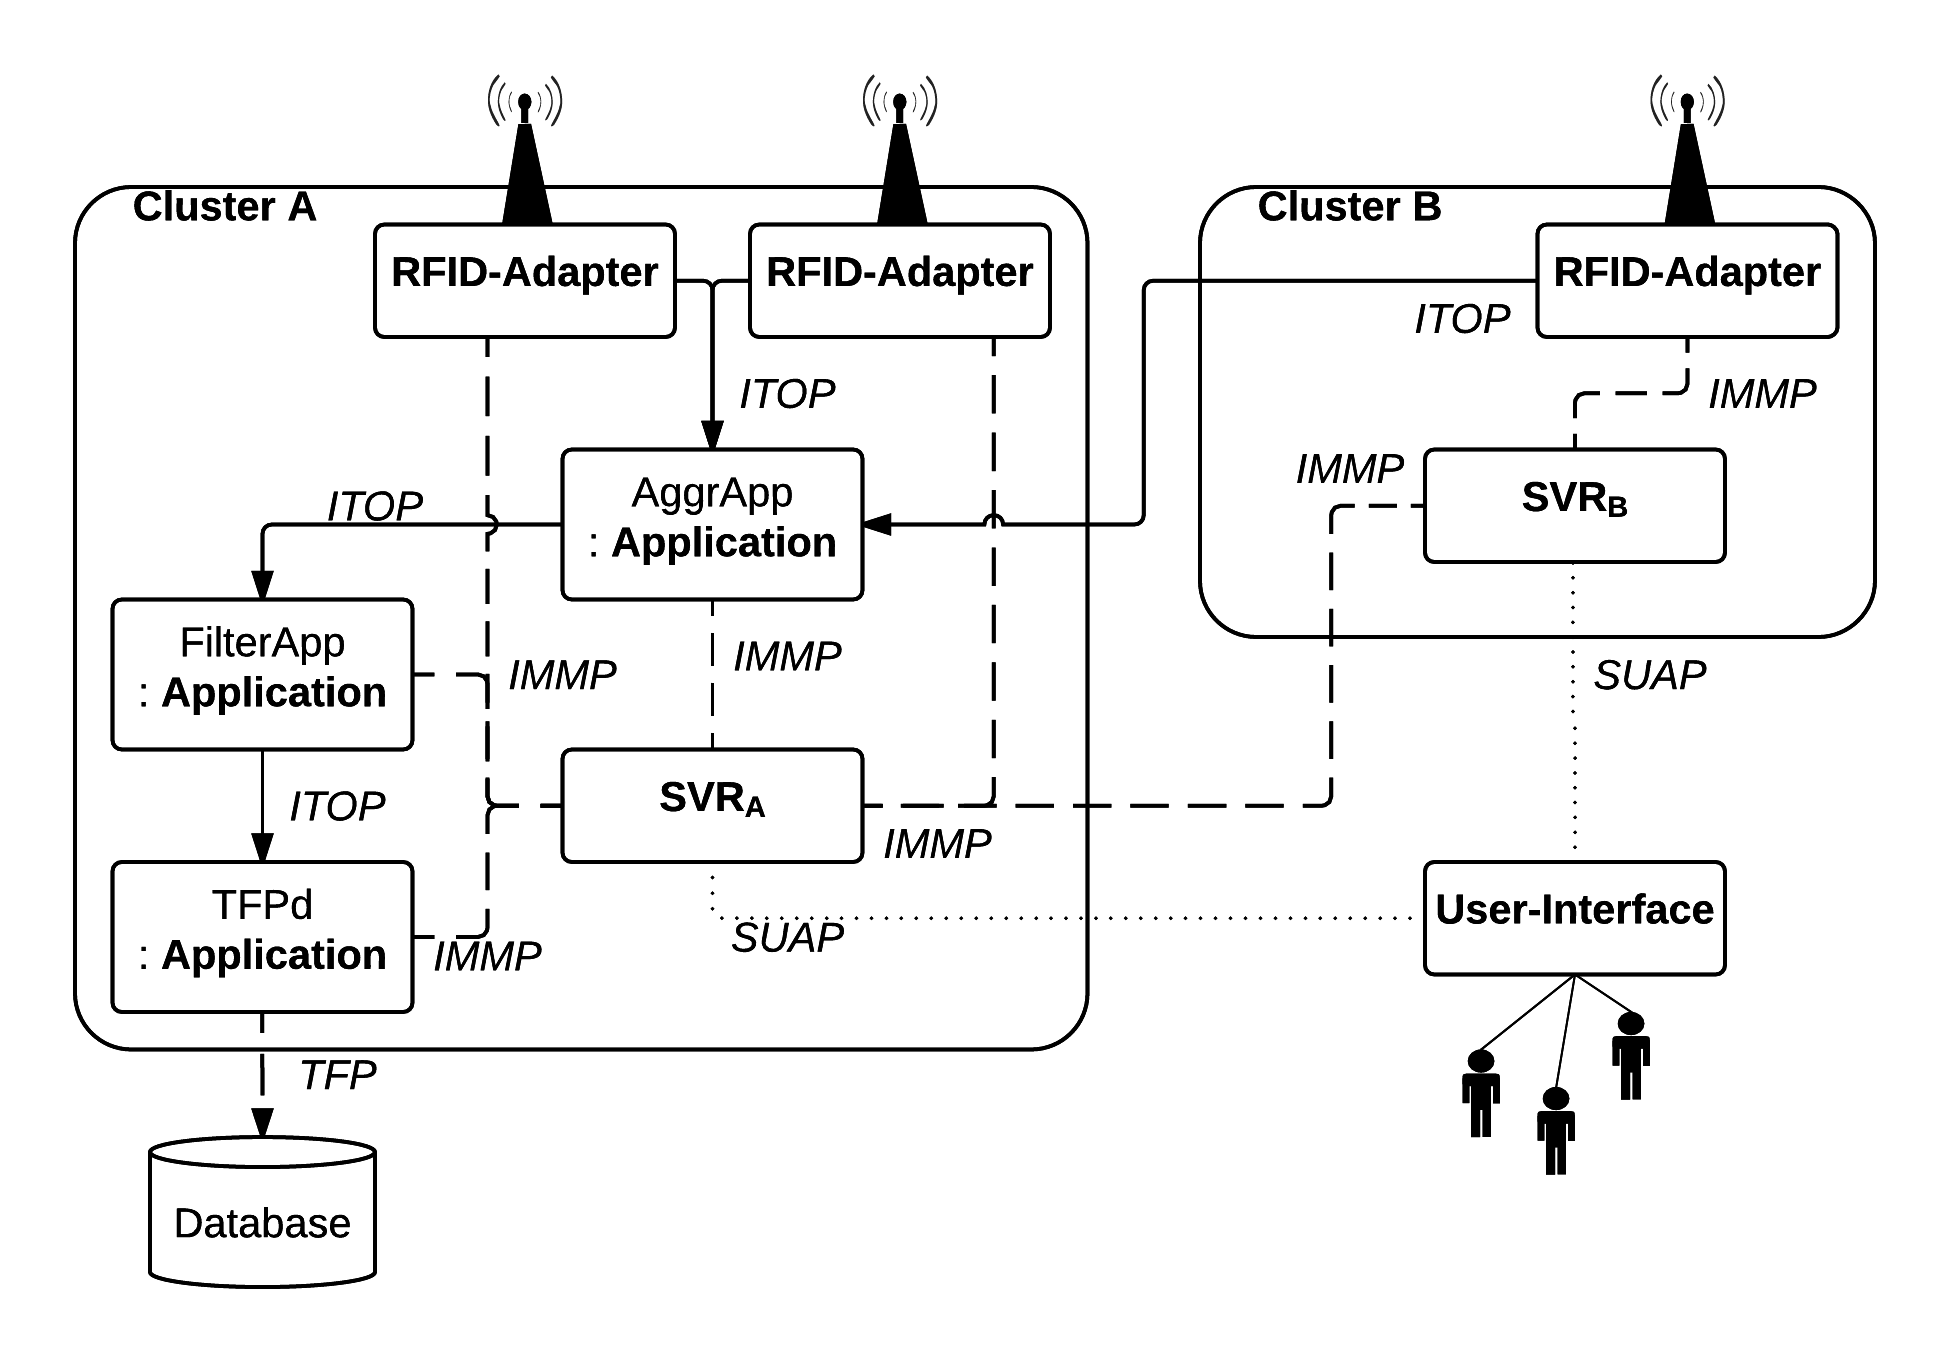
\includegraphics [width=0.7\textwidth]{chapter5/ch5_system_example}
  }
  \caption{Пример распределенной системы с двумя кластерами}
  \label{fig:ch5_system_example}
\end{figure}

Программная платформа состоит из трех типов компонентов, взаимодействующих по сети: управляющих модулей, называемых \textbf{супервайзерами} (SVR), \textbf{RFID-адаптеров}, осуществляющих работу со считывателями, а также \textbf{приложений}, реализующих ту или иную логику работы с адаптерами, обработку потоков прочитанных меток и выполняющих прочие функции. Пример платформы приведен на рис.~\ref{fig:ch5_system_example}.

\textbf{Супервайзеры} (SVR) отвечают за регистрацию, конфигурацию и мониторинг модулей, а также за авторизацию пользователей. Подсистема, состоящая из супервайзера и подключенных к нему модулей, называется \textit{кластером}. Модули взаимодействуют с SVR посредством специально разработанного протокола IMMP (см. раздел \ref{sec:ch5_immp}). Пользователи взаимодействуют с SVR с помощью другого протокола, также разработанного для использования внутри платформы, "--- SUAP (описан в разделе \ref{sec:ch5_suap}).

\textbf{RFID-адаптеры} "--- это программы--демоны, предоставляющие унифицированный интерфейс к считывателям. Каждый адаптер принимает запросы от прочих модулей, контролирует параметры настройки считывателя и реализует операции чтения/записи. Начальную конфигурацию адаптеры получают от супервайзера через протокол IMMP. Запросы на чтение и запись меток передаются адаптерам по протоколу ITOP, который будет более подробно рассмотрен в разделе \ref{sec:ch5_itop}. ITOP-соединения устанавливаются непосредственно между модулями, в отличие от IMMP-соединений, одной из сторон которых всегда является SVR. Цель такого разделения "--- позволить модулям получать данные от адаптеров независимо от SVR, значительно снижая тем самым нагрузку на супервайзер. Можно привести аналогию с независимой передачей сигнализации в IP-телефонии (например, в протоколе SIP) и передачей голосовых пакетов по протоколу RTP/RTCP "--- передача сигнализации идет через цепочку коммутаторов, а голос может передаваться через иные маршруты, соединяющие непосредственно пользовательские терминалы. Одна из главных особенностей протокола ITOP "--- поддержка потоковой передачи (стриминга) прочитанных меток: модули--клиенты могут подписываться на поток и получать все метки, считанные RFID-адаптером. Метки будут читаться до тех пор, пока последний подписчик не откажется от подписки (или соответствующее ITOP-соединение не будет завершено).

\textbf{Приложения} "--- это модули, осуществляющие обработку данных, поступающих от других модулей (адаптеров или приложений) через протокол ITOP. Модули--приложения направлены на решение различных задач: фильтрация потоков и их модификация, подключение к внешним базам данных, выполнение функций сетевых мостов (конверсия протоколов) и прочих функций.

Каждый компонент поддерживает множество \textbf{объектов}, каждый из которых является либо параметром, либо процедурой. Обработка объектов ведётся по запросам, приходящим от пользователей или других компонентов системы. Множество объектов полностью определяется типом компонента. Например, каждый RFID--адаптер поддерживает параметры <<температура радио--модуля>>, <<значение Q>>, <<номер сессии>> и процедуры <<выключить радио--модуль>>, <<включить радио--модуль>>. RFID--адаптер, специализированный на поддержке определенного считывателя, может также предоставлять специализированные объекты, специфичные для конкретной модели считывателя. Каждый модуль получает свои настройки от супервайзера при установке IMMP-соединения, которую он производит при запуске.

Для работы с объектом пользователь или системый модуль должны отправить запрос супервайзеру через SUAP или IMMP соответственно. Супервайзер поддерживает множество собственных объектов, например "--- <<число активных пользователей>> или <<статус подключений модулей>>. Также супервайзер выполняет проксирование объектов всех подключенных модулей, т.е. когда SVR получает запрос на объект, который не принадлежит самому SVR, он перенаправляет IMMP-запрос компоненту, которому этот объект принадлежит, и отвечает клиенту, перенаправляя ответ, полученный от компонента. Если объект принадлежит модулю, размещенному в другом кластере, SVR пересылает запрос супервайзеру нужного кластера.

Пользователи могут настраивать систему и взаимодействовать с RFID-адаптерами и приложениями. В системе определены четыре уровня доступа: наблюдатели, операторы, администраторы и суперпользователи. \textbf{Наблюдатели} могут подписываться на потоки меток, но не могут записывать метки или менять настройки оборудования. \textbf{Операторы} имеют право настраивать RFID--адаптеры и выполнять операции чтения/записи меток, однако не могут менять настройки остальных компонентов системы. \textit{Администраторы} имеют право настраивать модули, но не могут записывать метки. \textit{Суперпользователи} имеют права на любые действия с системой.

Помимо уровней доступа пользователей, с каждым компонентом связан специальный системный уровень доступа, который позволяет ему работать с определенным набором объектов других модулей. Например, приложения могут читать, но не имеют права записывать параметры RFID--адаптеров.

\begin{figure}[ht] 
  \centerfloat{
    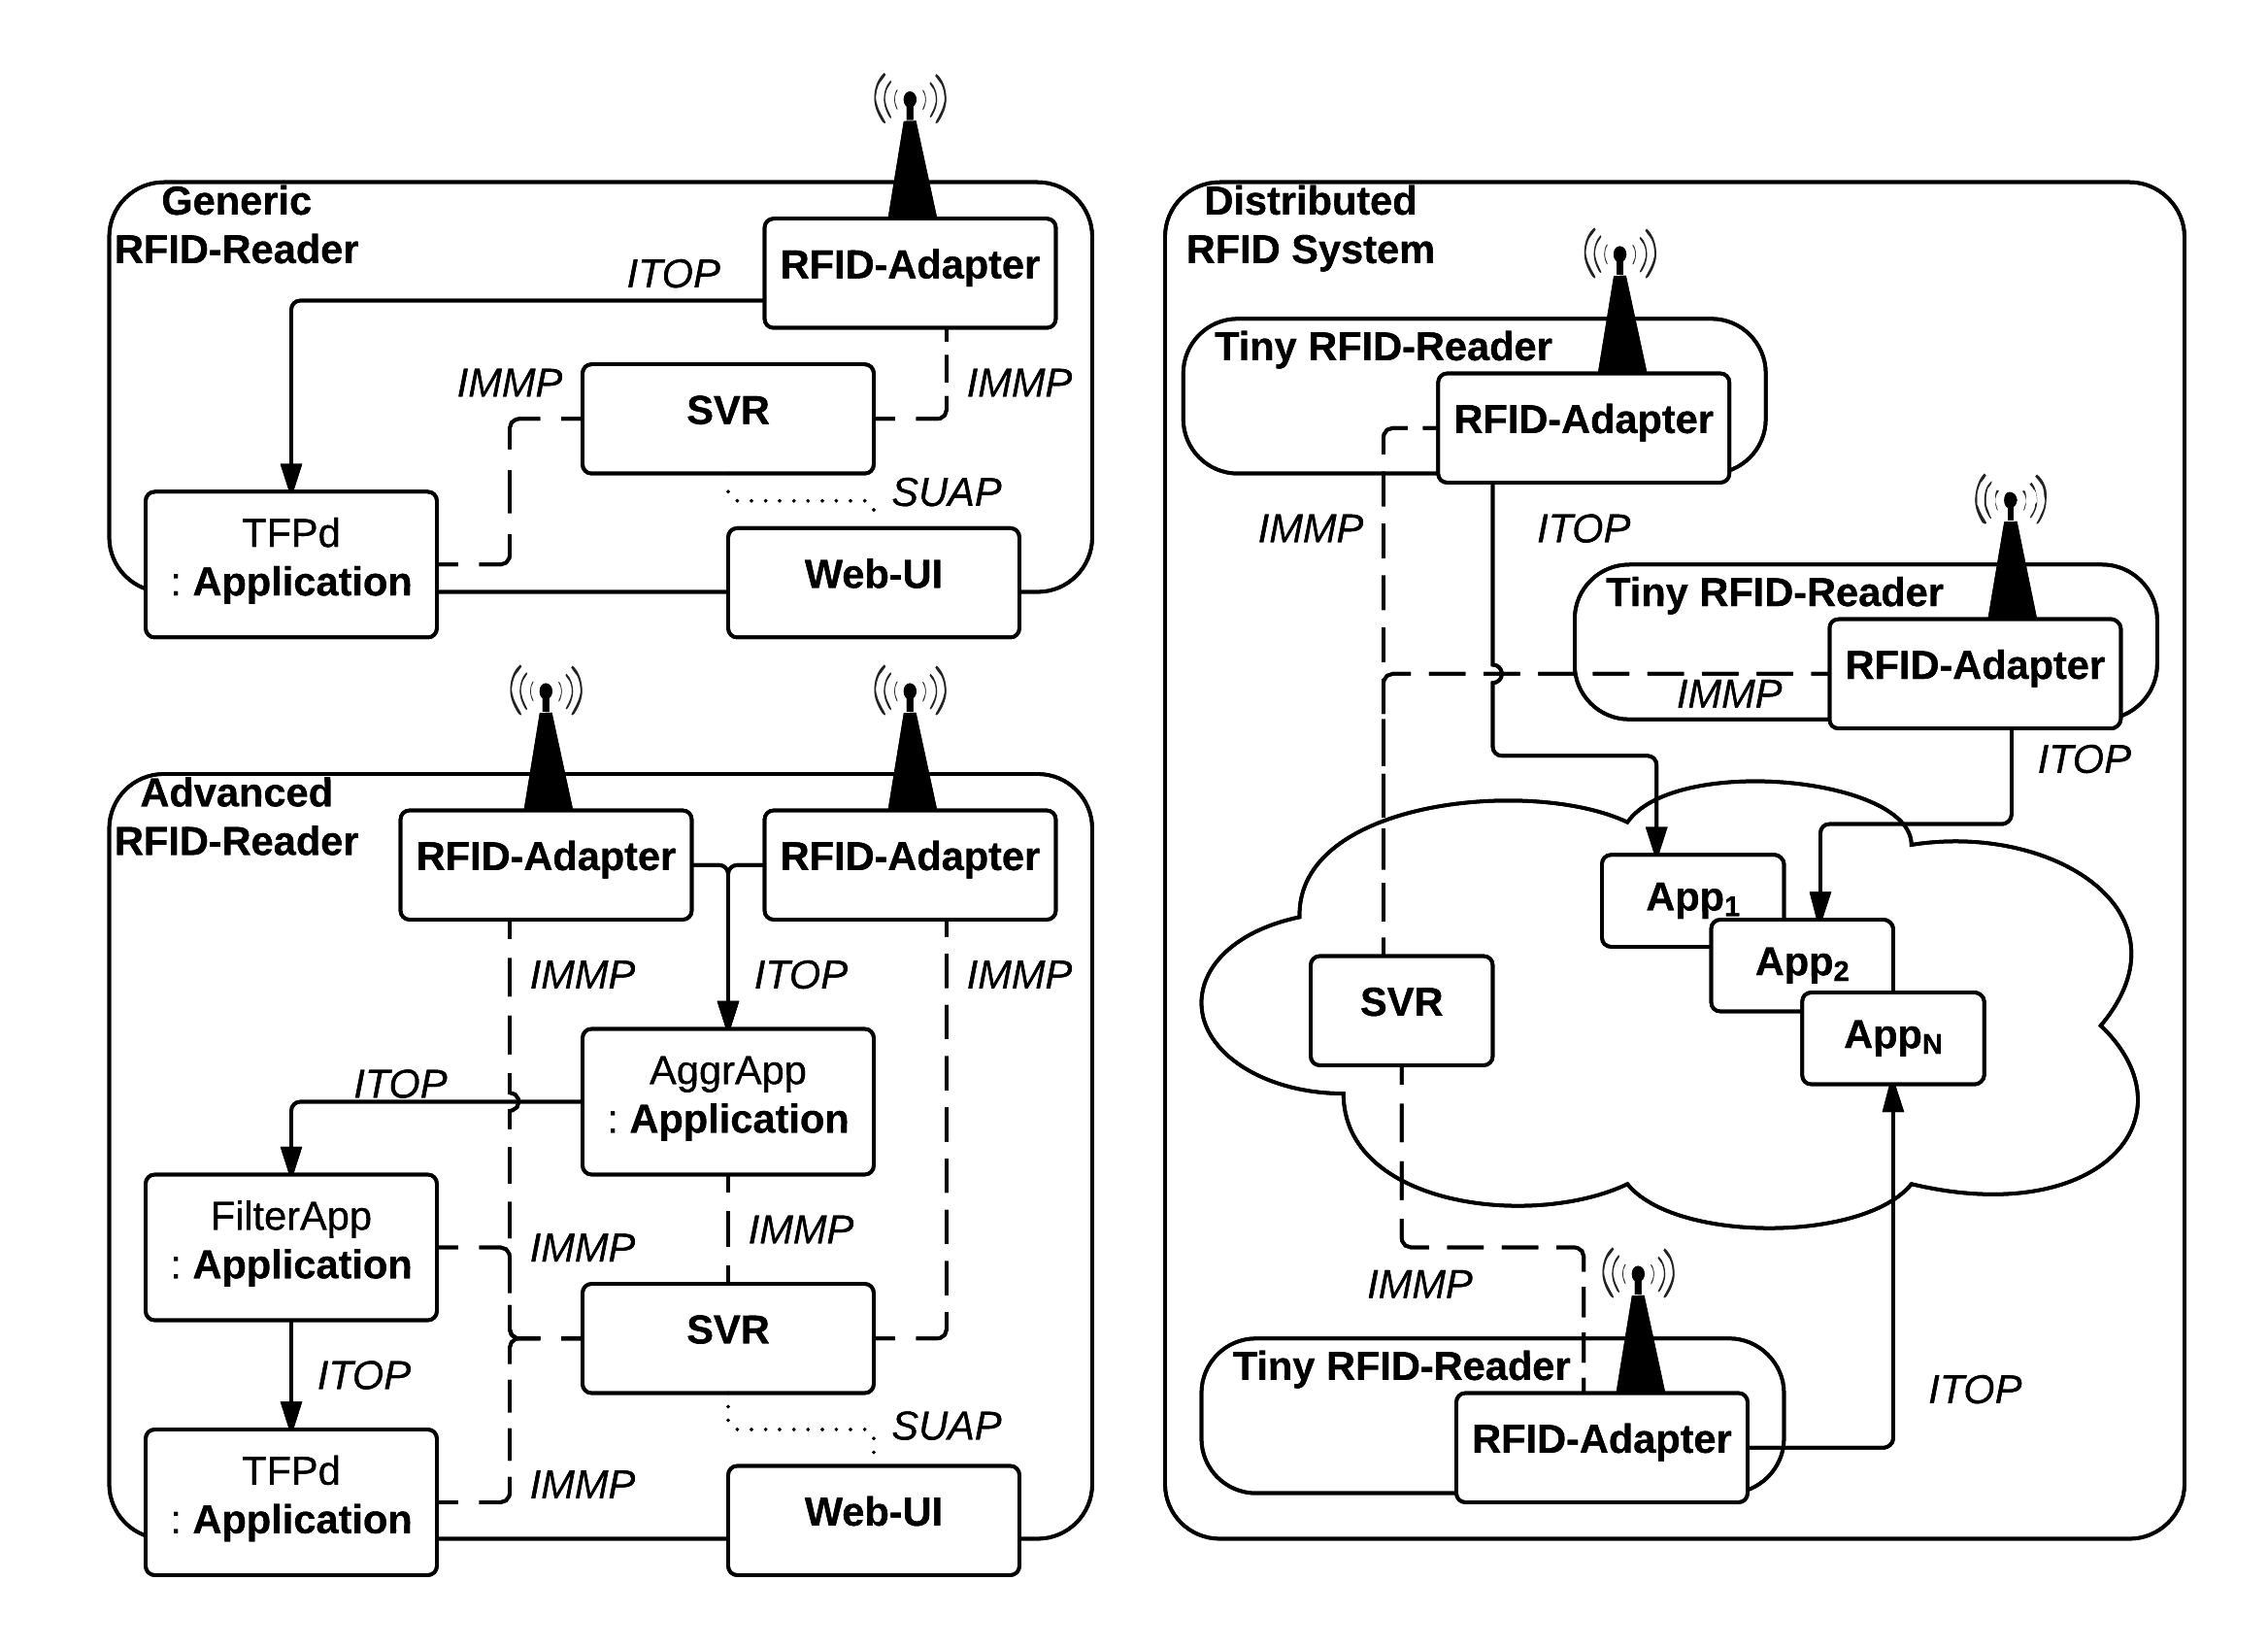
\includegraphics [width=0.9\textwidth]{chapter5/ch5_deployment_example}
  }
  \caption{Пример размещения компонентов системы}
  \label{fig:ch5_deployment_example}
\end{figure}

Поскольку все компоненты системы взаимодействуют друг с другом по сети, физически они могут располагаться где угодно. Типичные примеры размещений модулей по считывателям и серверам показаны на рис.~\ref{fig:ch5_deployment_example}.

Для обычного RFID--считывателя, построенного на базе среднего процессора (например, одноядерный ARM A7 или ARM A8), обладающего небольшим объемом оперативной памяти порядка 256--512~МБ и имеющего в составе один радиомодуль, достаточно установить SVR, RFID-адаптер, а также приложение для подключения к потоку прочитанных меток снаружи (TFPd) и модуль, предоставляющий доступ к настройке считывателю через web-интерфейс или консоль. Такое размещение компонентов позволяет передавать данные о всех прочитанных метках в центр обработки данных и, при необходимости, реализовывать операции чтения/записи через подключение внешних модулей и пользователей по протоколам ITOP и SUAP. Именно такая конфигурация считывателей использовалась в эксперименте, проведенном в городе Казань.

Если считыватель имеет более мощное вычислительное ядро, на нём также можно разместить несколько приложений (например, для фильтрации прочитанных меток или объединения с данными, получаемыми от другого считывателя). Если считыватель включает несколько радиомодулей, то также потребуется размещение несольких RFID--адаптеров. Хотя каждый компонент системы не требователен к вычислительным ресурсам по отдельности, для выполнения задач обработки поток меток могут потребоваться дополнительные ресурсы. Желательно использовать 2-х или 4-х ядерный процессор ARM и 512 "--- 1024 МБ оперативной памяти.

В наиболее сложном случае система может работать в распределенном режиме, а различные ее компоненты размещаться на считывателях и серверах, при этом считыватели могут быть сделаны чрезвычайно <<тонкими>> "--- на них достаточно разместить RFID--адаптер, который будет подключаться по сети к SVR, работающему на внешнем сервере. Приложения также могут работать на отдельных физических или виртуальных внешних серверах. В этом варианте считыватели могут быть реализованы на самых простых вычислительных компонентах, что позволит снизить их стоимость. При этом приложения и SVR выполняются в центре обработки данных, на мощном вычислительном оборудовании, благодаря чему им можно поручить работу с большим числом считывателей и выполнение достаточно сложных функций. Такой вариант размещения наиболее гибок и позволяет построить распределенную систему, состоящую из сотен считывателей, каждый из которых может администрироваться из единой консоли администратора. Добавление нового считывателя реализуется просто: администратор должен прописать адрес SVR в настройках RFID--адаптера, а также настроить приложения на работу с этим считывателем.



%%%%%%%%%%%%%%%%%%%%%%%%%%%%%%%%%%%%%%%%%%%%%%%%%%%%%%%%%%%%%%%%%%%%%%%%%%%%%%%%
\section{Протоколы взаимодействия компонентов системы}\label{sec:ch5_protocols}
%%%%%%%%%%%%%%%%%%%%%%%%%%%%%%%%%%%%%%%%%%%%%%%%%%%%%%%%%%%%%%%%%%%%%%%%%%%%%%%%

Для работы распределенной системы были разработаны четыре протокола:

\begin{itemize}
\item{\textit{IMMP} (\textit{Internal Modules Management Protocol}): протокол, используемый компонентами системы для подключения к SVR. Позволяет передавать начальную конфигурацию модулям, предоставляет возможность получения и установки значений объектам--параметрам и обеспечивает возможность вызова объектов--процедур. Протокол работает поверх TCP.}
\item{\textit{SUAP} (\textit{Simple User Access Protocol}): подключает пользователей к SVR, предоставляет возможность получения и установки значений параметров и удаленного вызова процедур. Работает через UDP.}
\item{\textit{ITOP} (\textit{Internal Tags Operation Protocol}): предоставляет соединения между компонентами для передачи данных о считанных метках, а также позволяет записывать метки и выполнять с ними прочие операции. Содержит механизмы для подписывания на поток считанных меток.}
\item{\textit{TFP} (\textit{Tag Flow Protocol}): упрощенная версия ITOP, предоставляющая возможность создания подписки на поток считанных меток. Может использоваться для подключения внешних приложений "--- например, клиента, записывающего поток меток в базу данных или клиента, записывающего данные во внутренний кэш для последующей выгрузки во внешние базы.}
\end{itemize}

Все протоколы имеют клиент--серверную архитектуру, соединение создаётся клиентом. Каждый запрос должен подтверждаться получателем с помощью специального сообщения \texttt{Response}, содержащего результат обработки запроса или код ошибки. Запросы упорядочиваются с помощью порядкового номера \texttt{ReqSN} (Request Sequence Number): клиент и сервер поддерживают по счетчику, перед отправкой значение счетчика увеличивается и помещается в соответствующее поле в запросе. В ответе на запрос поле \texttt{ReqSN} должно совпадать со значением счетчика из запроса. Этот механизм позволяет реализовать асинхронную обработку запросов "--- отправителю запроса не нужно ждать ответа для того, чтобы передать новый запрос. При этом отправитель может быть уверен, что запросы будут обработаны в порядке их передачи: если получатель видит, что номер запроса меньше последнего обработанного, запрос будет проигнорирован. С каждым запросом также связано максимальное ожидание ответа, после которого отправитель считает, что запрос не был выполнен.

Формат сообщений, кодируемых с помощью ASCII-строк, аналогичен форматам, используемым в HTTP v1.1 и SIP.


%%% --------------------------------------------
\subsection{Протокол управления платформой (IMMP)}\label{sec:ch5_immp}
%%% --------------------------------------------

\begin{figure}[ht] 
  \centerfloat{
    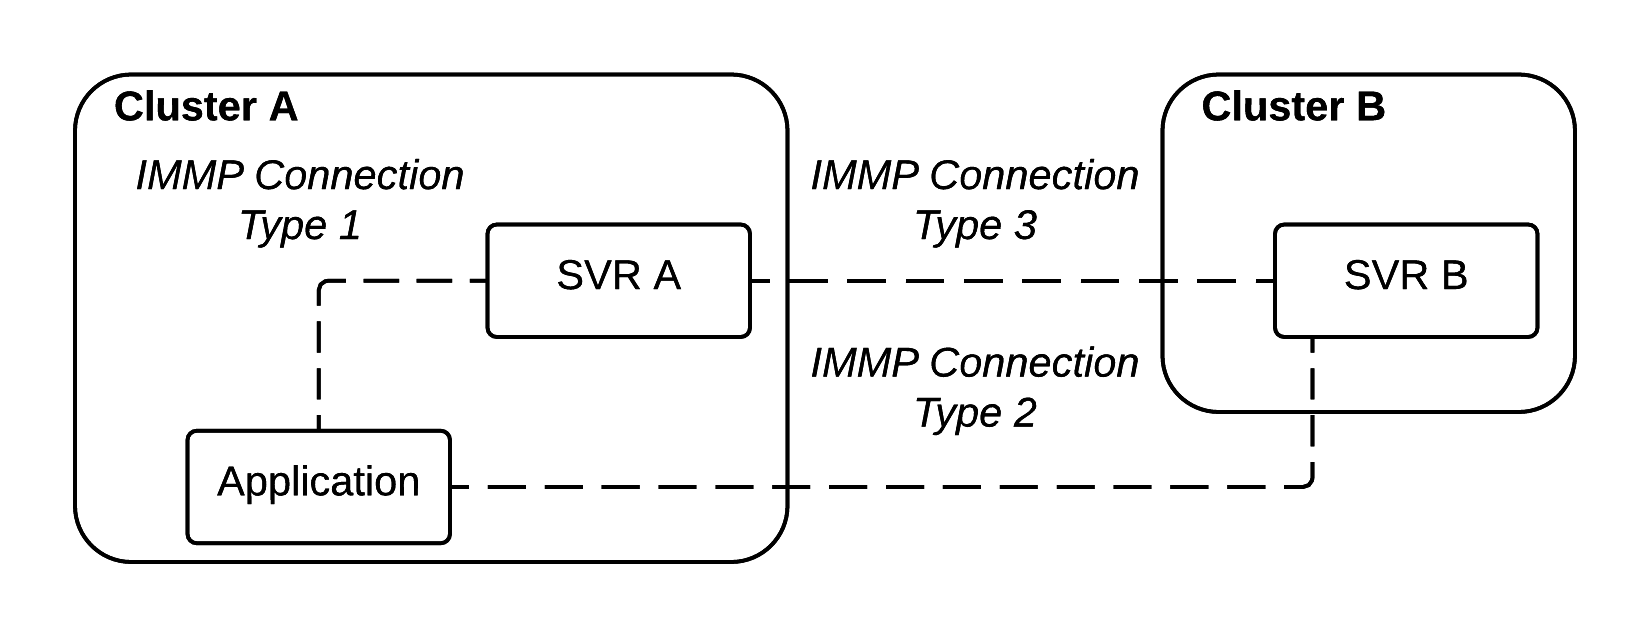
\includegraphics [width=0.8\textwidth] {chapter5/ch5_immp_connections}
  }
  \caption{Примеры IMMP-соединений}
  \label{fig:ch5_immp_connections}
\end{figure}

Протокол IMMP работает поверх транспортного уровня TCP и реализует функции получения модулями своей начальной конфигурации от супервайзера, поиск IP-адреса модуля по имени (сервис локации), получение и установка значений объектов, а также удалённый вызов процедур. В рамках IMMP различаются три типа соединений (см. рис.~\ref{fig:ch5_immp_connections}):

\begin{itemize}
	\item Тип 1: соединения между модулем с SVR из того же кластера. В этом соединении могут передаваться любые запросы, получение стартовой конфигурации модулем осуществляется через это соединение. В роли клиента всегда выступает модуль, подключаемый к SVR.
	\item Тип 2: соединения между модулем с SVR из другого кластера. Схоже с соединением типа 1, но не предполагает передачу стартовой конфигурации и может содержать ограничения на установку значений параметров и вызов процедур. Как и в соединении типа 1, в роли клиента всегда выступает модуль, подключаемый к SVR.
	\item Тип 3: соединения между SVR из разных кластеров. Предназначен для настройки SVR-клиента, инициализирующего соединение, через SVR--сервер. Предполагается, что SVR может поддерживать не более одного соединения типа 3 в качестве клиента, и сколько угодно --- в качестве сервера.
\end{itemize}

В протоколе определены семь запросов: \texttt{HELLO}, \texttt{ACK}, \texttt{BYE}, \texttt{LOCATE}, \texttt{GET}, \texttt{SET} и \texttt{CALL}. Запрос \texttt{HELLO} отправляется клиентом для создания соединения. Если соединение может быть установлено, сервер (SVR) сначала передает \texttt{Response} с кодом успеха (200), а затем "--- запрос \texttt{ACK}, в котором передает параметры сессии, включая ключ сессии \texttt{SKey} (Session Key). Запрос \texttt{LOCATE} используется для поиска компонентов по их именам или типам. Запросы \texttt{GET} и \texttt{SET} используются для чтения и записи значений объектов--параметров, а запрос \texttt{CALL} "--- для удаленного вызова процедур. Запросы \texttt{GET}, \texttt{SET} и \texttt{CALL} могут передаваться как клиентом, так и сервером.

\begin{figure}[ht] 
  \centering
  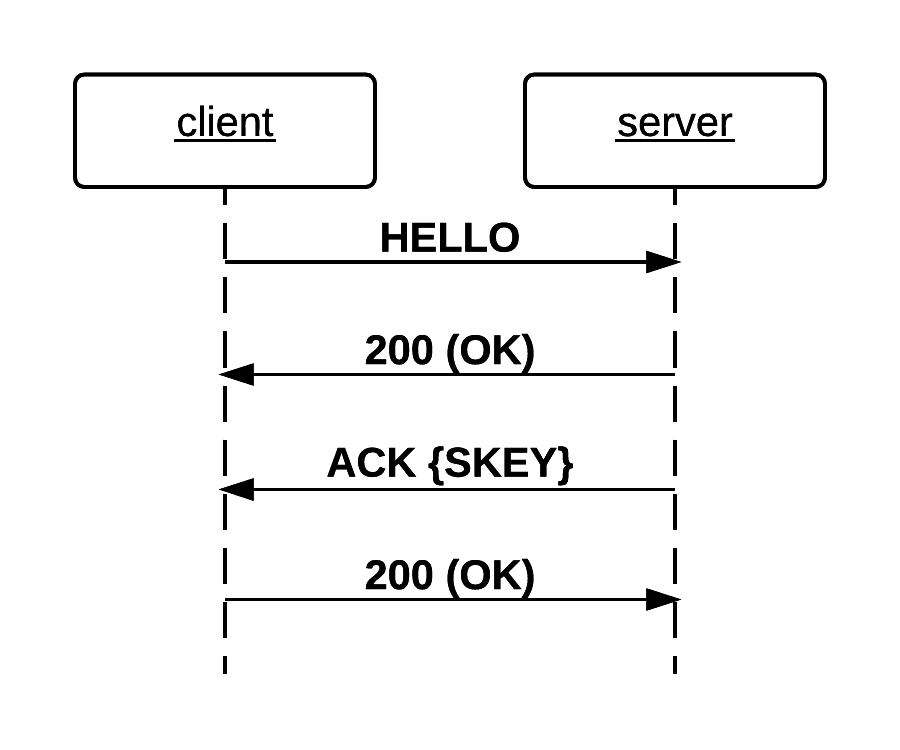
\includegraphics [width=0.4\textwidth] {chapter5/ch5_immp_session_establishment}
  \caption{Создание IMMP-соединения}
  \label{fig:ch5_immp_session_establishment}
\end{figure}

Создание соединения показано на рис.~\ref{fig:ch5_immp_session_establishment}. Клиент передает запрос \texttt{HELLO} со своим типом и именем. Сервер передает ответ \texttt{Response} с кодом 200. Затем сервер готовит стартовую конфигурацию клиента и передает ее в запросе \texttt{ACK}, получение которого также должен подтвердить клиент отправкой \texttt{Response}. Такое разделение ответов сервера возникает из-за того, что при высокой нагрузке на SVR подготовка стартовой конфигурации может занять время, которое может превышать время ожидания ответа на запрос \texttt{HELLO}. После получения ответа на \texttt{HELLO} клиент может ждать гораздо дольше получения своей конфигурации в \texttt{ACK}. Помимо начальной конфигурации, в \texttt{ACK} супервайзер передает ключ сессии \texttt{SKey}, который используется в дальнейшем обмене сообщениями. Хотя при использовании постоянных соединений TCP этот ключ представляет собой скорее рудимент, в будущем предполагается возможность использования на транспортном уровне протокола UDP, а в этом случае использование ключа позволяет идентифицировать запрос с сеансом.

Если одному компоненту нужен адрес другого компонента (например, для создания ITOP-соединения), он передает запрос \texttt{LOCATE} своему SVR. Если компонент найден, SVR передает его адрес в ответе на \texttt{LOCATE}. Если SVR не может найти компонент среди своих подключений, он может передать запрос по соединениям типа 3 для поиска компонента в других кластерах.

Если SVR нужно выполнить какую-либо операцию над объектом другого компонента, он передает соответствующий запрос (\texttt{GET}, \texttt{SET} или \texttt{CALL}). Если же компоненту A нужно выполнить действие над объектом компонента B, то SVR выступает в роли прокси-сервера: компонент A передает запрос SVR, который SVR передает компоненту B, дожидается ответа и пересылает его компоненту A.

Одно из приемуществ использования IMMP для управления компонентами системы "--- возможность быстрого изменения расположения компонентов. Если приложению нужно установить соединение, например, с RFID-адаптером, он запрашивает его адрес с помощью запроса \texttt{LOCATE}, в котором использует символьное имя этого адаптера (или, если ему нужно подключиться ко всем адаптерам, достаточно указать тип). В ответе SVR сообщит адрес (или адреса), по которым приложение уже может подключаться к адаптерам.



%%% --------------------------------------------
\subsection{Протокол подключения интерфейсов управления (SUAP)}\label{sec:ch5_suap}
%%% --------------------------------------------

Протокол SUAP представляет собой упрощенную версию IMMP, работающую через UDP. Он предназначен для подключения пользовательских интерфейсов к SVR. В функции SUAP входят получение и установка значений параметров, удаленный вызов процедур и обнаружение компонентов. Предполагается, что модули, предоставляющие пользователям доступ, не имеют своих объектов, поэтому передавать им начальную конфигурацию не надо, соответственно, отсутствует запрос \texttt{ACK}. По этой же причине протокол не является симметричным "--- запросы \texttt{GET}, \texttt{SET} и \texttt{CALL} могут передаваться только от клиента серверу. Ключ сессии \texttt{SKey} необходим для идентификации клиента и сессии и, ввиду отсутствия \texttt{ACK}, передается SVR клиенту в ответе на запрос \texttt{HELLO}.

Так как SUAP работает через UDP, в нем присутствует механизм для отслеживания состояния соединений: если сервер не получает от клиента ни одного сообщения в течение определенного интервала (по-умолчанию, 10 минут), он считает, что клиент отключился и сессия завершается. Для предотвращения этой ситуации, клиент может периодически передавать специальные короткие запросы \texttt{KEEPALIVE}, если передавать содержательные запросы ему не нужно.



%%% --------------------------------------------
\subsection{Протокол работы с RFID-адаптерами (ITOP)}\label{sec:ch5_itop}
%%% --------------------------------------------

Протокол предназначен для связи между компонентами системы (приложениями и RFID-адаптерами), желающими осуществлять действия над метками. Он позволяет читать и записывать память меток, а также подписываться на потоки считанных меток. Подписка может быть позднее отменена, также она завершается при закрытии соединения любой из сторон.

В протоколе определены семь запросов: \texttt{HELLO}, \texttt{READMEM}, \texttt{WRITEMEM}, \texttt{WRITEEPC}, \texttt{SUBSCRIBE}, \texttt{UNSUBSCRIBE} и \texttt{BYE}. Запросы \texttt{HELLO} и \texttt{BYE} используются для создания и завершения соединений соответственно, причем запрос \texttt{HELLO} может передаваться только клиентом, а \texttt{BYE} "--- любой из сторон. \texttt{SUBSCRIBE} и \texttt{UNSUBSCRIBE} передаются клиентом и используются для создания и отмены подписки соответственно. Запросы \texttt{READMEM}, \texttt{WRITEMEM} и \texttt{WRITEEPC} передаются клиентом для чтения или записи данных на заданную метку.

В протоколе ITOP также определен специальный вид сообщения--ответа \texttt{NOTIFY}. Это сообщение асинхронно передаётся сервером для информирования клиента, подписавшегося на поток, о прочтении новой метки. Он содержит следующие поля:

\begin{itemize}
	\item \texttt{epc}: значение EPC прочитанной метки;
	\item \texttt{tid}: значение банка TID прочитанной метки;
	\item \texttt{um}: значение банка UserMemory прочитанной метки;
	\item \texttt{id}: значение идентификатора метки, определенного приложением;
	\item \texttt{rssi}: мощность принятого сигнала;
	\item \texttt{antenna}: номер антенны RFID-считывателя, на которой была считана метка;
	\item \texttt{source}: имя RFID-адаптера, который изначально считал метку;
	\item \texttt{count}: число раз, которое метка была считана.
\end{itemize}

Идентификатор \texttt{id} заполняется данными, специфичными для приложения. Оно может содержать значение EPC или некоторое значение, полученное приложением с помощью EPC, TID, UserMemory. Например, в роли идентификатора может выступать номер транспортного средства, полученный приложением посредством обращения к базе данных.

Когда клиент хочет установить ITOP-соединение, ему требуется обнаружить ITOP-сервер. Если клиент знает имя сервера, но не знает его IP-адрес, он передает запрос \texttt{LOCATE} на SVR через IMMP или SUAP и получает адрес сервера в ответе. Зная адрес, клиент создает с ним TCP-соединение и передает запрос \texttt{HELLO}. В запрос \texttt{HELLO} также включается значение \texttt{SKey}, полученный клиентом ранее, при создании IMMP- или SUAP--соединения. Значение \texttt{SKey} используется для авторизации сервером клиента на выполнение той или иной операции. Например, администраторы и наблюдатели не имеют права записывать метки, а единственная разрешенная им операция "--- создание подписки на получение потока меток.

\begin{figure}[ht] 
  \centerfloat{
    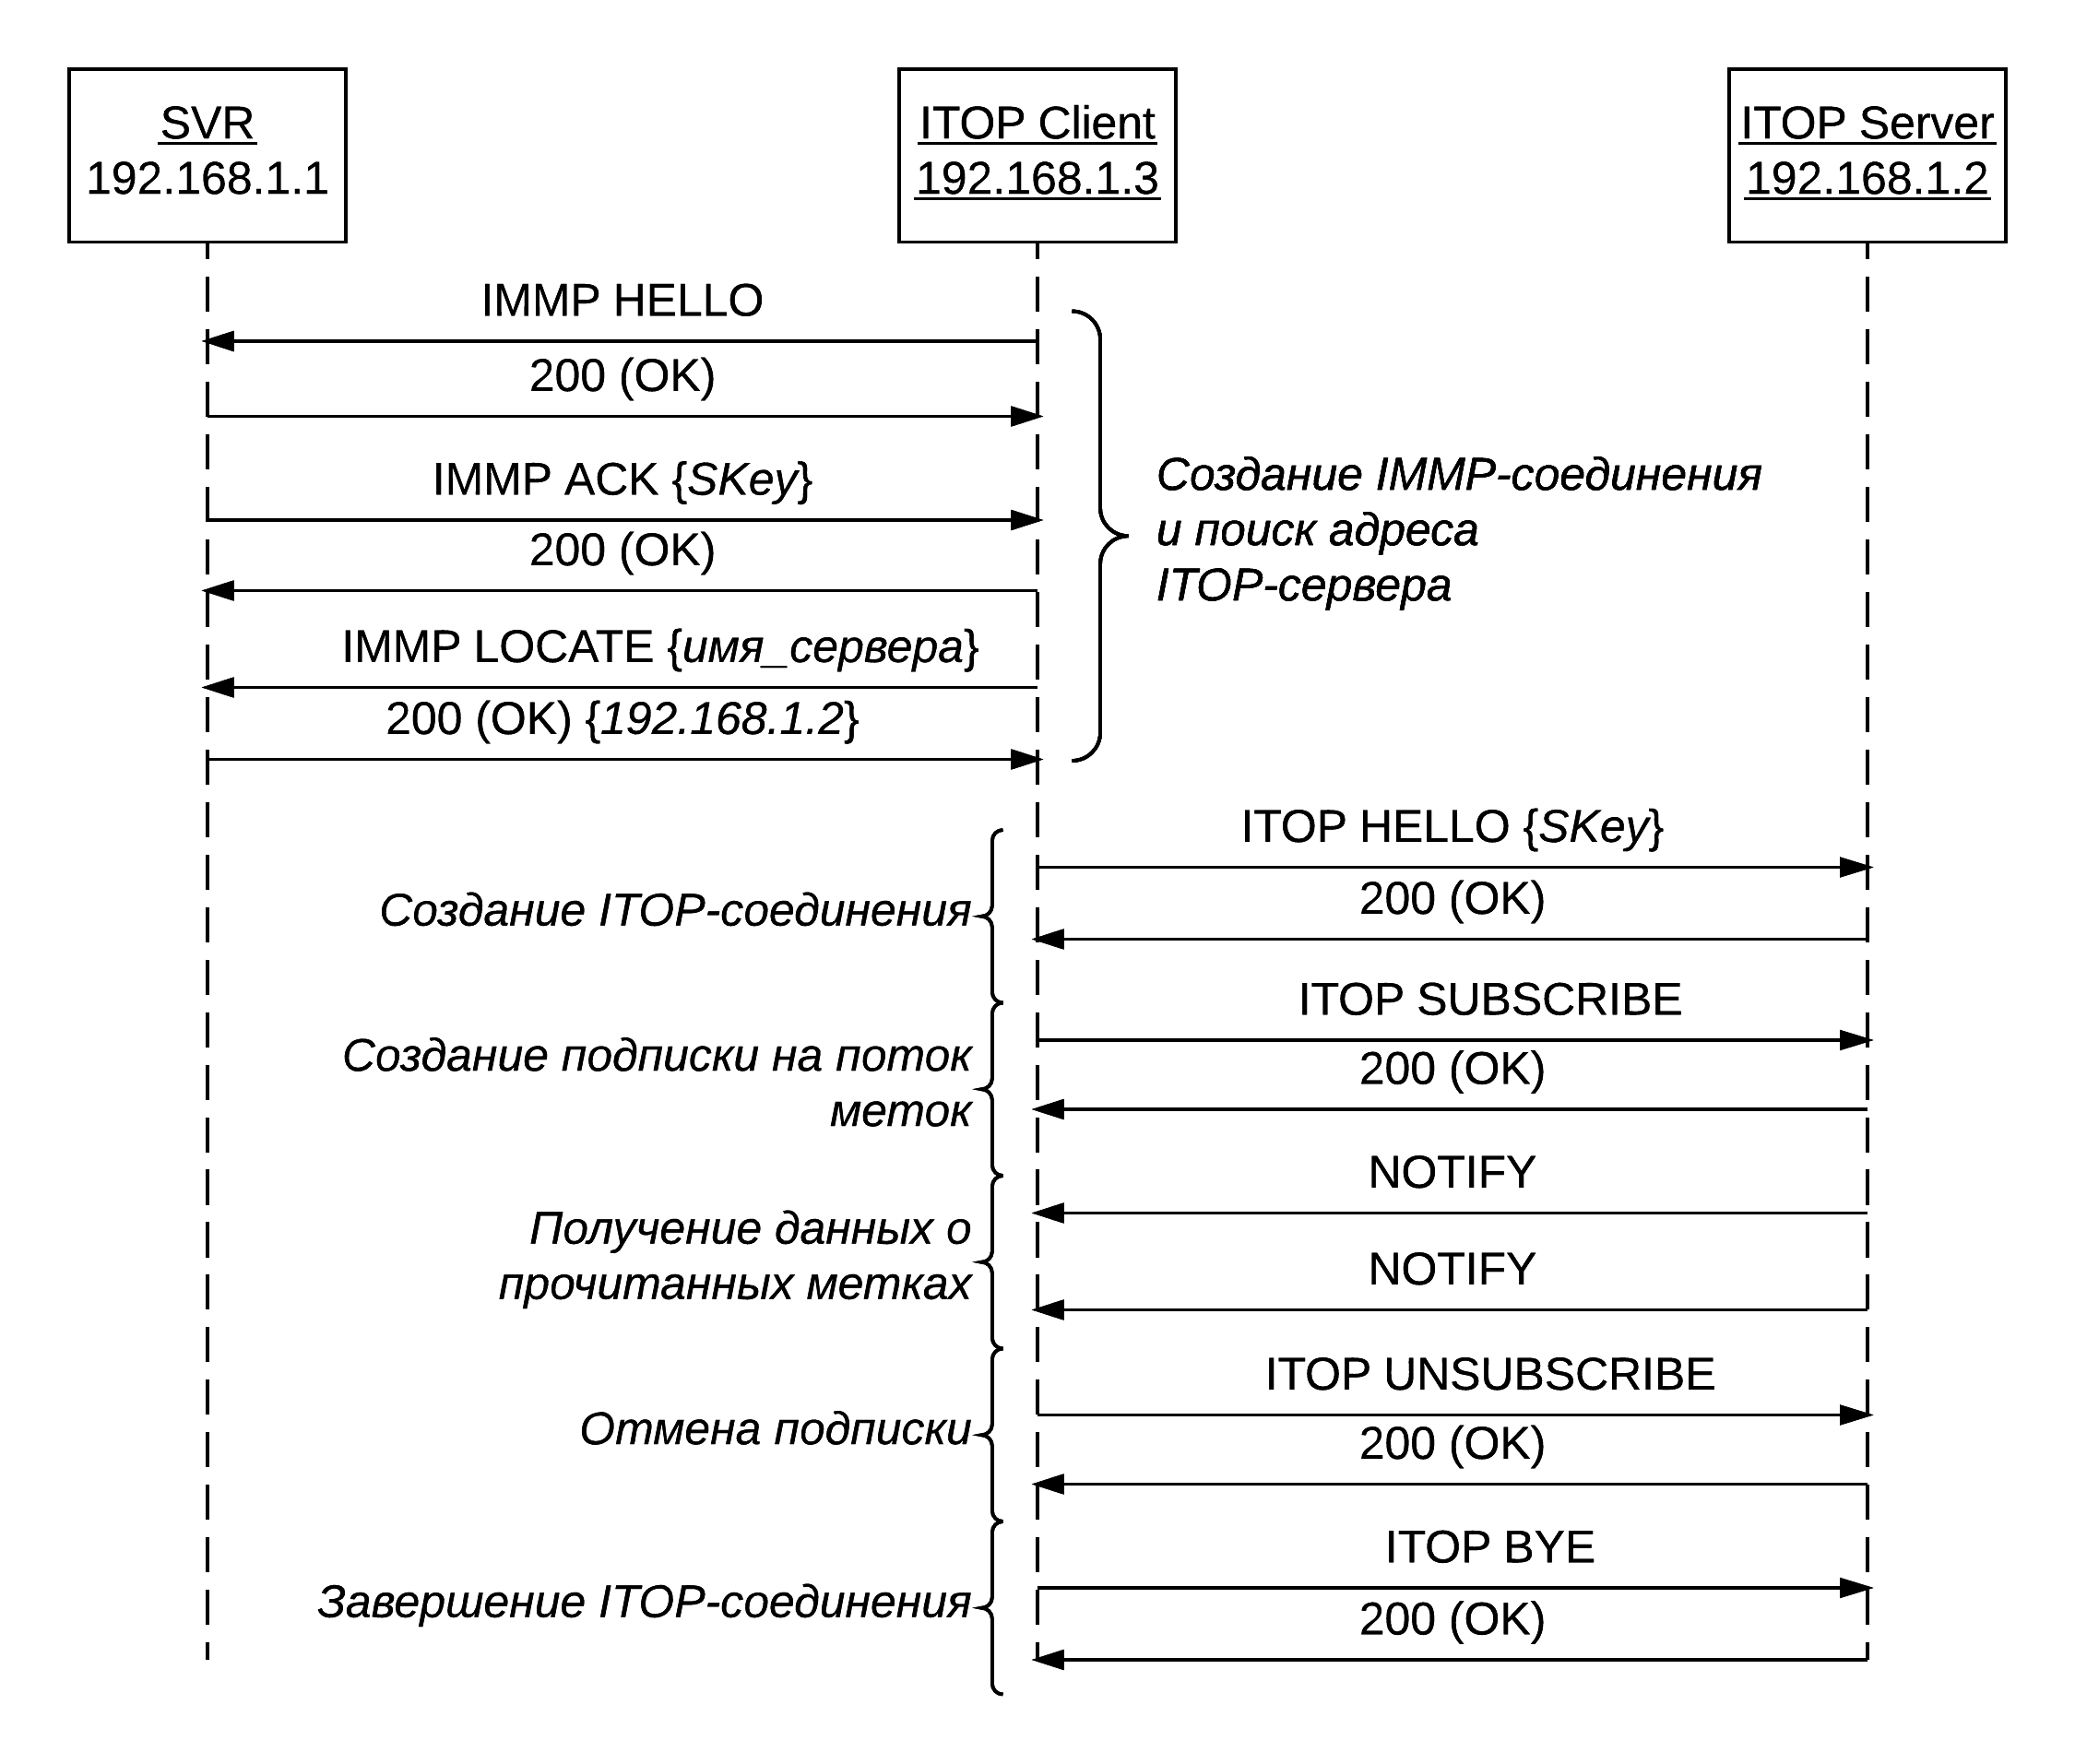
\includegraphics [width=0.8\textwidth] {chapter5/ch5_itop_session}
  }
  \legend{Клиент подключается по IMMP к SVR и получает ключ сессии \texttt{SKey}, затем запрашивает адрес ITOP-сервера. Получив адрес, клиент создает соединение с ITOP-сервером с использованием ключа \texttt{SKey}, создает подписку на получение меток. После получения двух меток клиент отменяет подписку и завершает соединение.}
  \caption{Пример ITOP-сессии}
  \label{fig:ch5_itop_session}
\end{figure}

Если клиент желает непрерывно получать информацию о прочитанных метках от сервера, он передает запрос \texttt{SUBSCRIBE}. Как только считывается (если сервер "--- RFID-адаптер) или принимается (если сервер "--- приложение) новая метка, сервер передает сообщение \texttt{NOTIFY} клиенту, содержащее информацию о метке. Когда клиент желает остановить получение потока, он отменяет подписку передачей запроса \texttt{UNSUBSCRIBE}. Пример сессии с показан на рис.~\ref{fig:ch5_itop_session}


%%% --------------------------------------------
\subsection{Протокол потокового чтения меток (TFP)}\label{sec:ch5_tfp}
%%% --------------------------------------------

Протокол TFP является упрощенной версией протокола ITOP и предназначен для получения данных о метках из пользовательских интерфейсов или внешних клиентов. Специальное приложение TFP Daemon (TFPd) реализует TFP-интерфейс и выступает в роли моста между ITOP и TFP: с одной стороны это приложение выступает в роли сервера протокола TFP, с другой "--- клиента ITOP. В протоколе TFP поддерживается только механизм создания подписок, прочие функции (запись меток, чтение заданных областей памяти и пр.) он не реализует. Кроме того, в сообщении \texttt{HELLO} не передается ключ сессии \texttt{SKey}, так как приложение TFPd использует свой собственный (системный) уровень доступа для создания ITOP-соединения с источником данных, позволяющий создавать подписки.



%%%%%%%%%%%%%%%%%%%%%%%%%%%%%%%%%%%%%%%%%%%%%%%%%%%%%%%%%%%%%%%%%%%%%%%%%%%%%%%%
\section{Приложения в программной платформе}\label{sec:ch5_applications}
%%%%%%%%%%%%%%%%%%%%%%%%%%%%%%%%%%%%%%%%%%%%%%%%%%%%%%%%%%%%%%%%%%%%%%%%%%%%%%%%

Кратко рассмотрим основные приложения, использующиеся в системе: агрегатор потоков AggrApp и TFP-сервер TFPd и кэш CacheApp. Работа этих приложений показана на рис.~\ref{fig:ch5_applications_scheme}.

\begin{figure}[ht] 
  \centerfloat{
    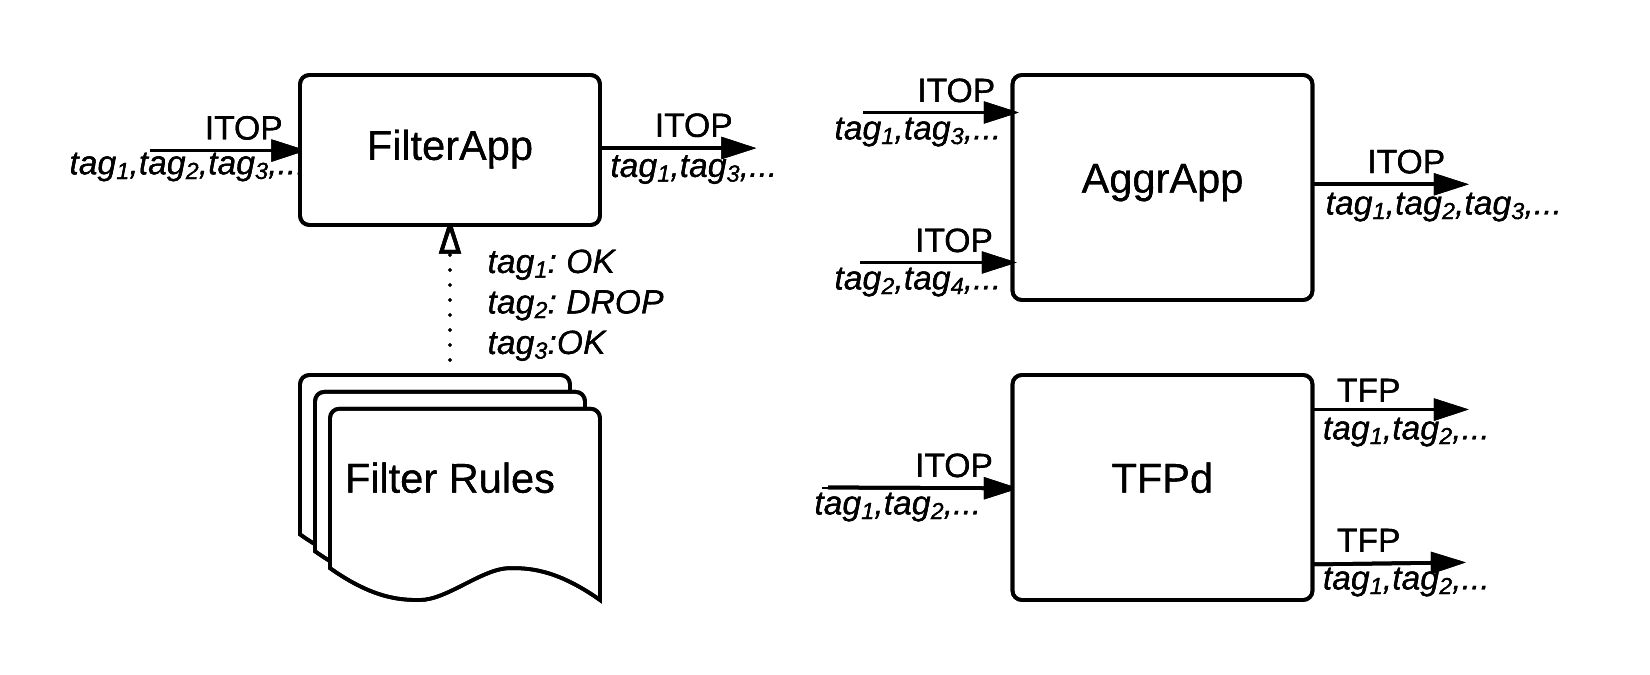
\includegraphics [width=0.85\textwidth] {chapter5/ch5_applications_scheme}
  }
  \caption{Приложения в программной платформе}
  \label{fig:ch5_applications_scheme}
\end{figure}

В дальнейшем могут быть реализованы более сложные приложения: фильтрация и модификация потока меток, преобразование протоколов (например, для подключения к платформе по протоколу web sockets), поиск номеров автомобилей по меткам в реальном времени и прочие.


%%% --------------------------------------------
\subsection{Агрегация потоков (AggrApp)}
%%% --------------------------------------------

Большинство приложений может подключаться к единственному ITOP-потоку. Если нужно объединить данные, поступающие от двух или более источников данных, можно использовать приложение AggrApp. Его функция "--- пересылка всем клиентам каждого \texttt{NOTIFY}-сообщения, поступающего в любом из входящих ITOP-соединений. Это единственное из приложений, имеющих множественный вход и множественный выход.

Приложение AggrApp создает подписки у своих источников данных только тогда, когда к нему подключается и создает подписку первый клиент. Если ни один клиент не подписан на поток от приложения, само приложение также не инициирует подписку.


%%% --------------------------------------------
\subsection{TFP-сервер и кэш}
%%% --------------------------------------------

Компоненты внутри системы используют протокол ITOP для чтения и записи меток. В то же время, для подключения внешних клиентов (например, для записи данных о проездах в базу данных в центре обработки данных) не нужны все функции ITOP. В частности, не нужно (и даже не желательно) иметь возможность записывать метки из ЦОДа. Для упрощения таких задач используется протокол TFP, который был рассмотрен ранее "--- в отличие от ITOP, он предоставляет возможность только для управления подпиской на поток данных о прочитанных метках.

Для того, чтобы преобразовать поток данных о прочитанных метках, получаемый от адаптеров или других приложений по протоколу ITOP, в TFP-поток, применяется приложение TFPd. При подключении первого клиента и создания этим клиентом подписки, TFPd связывается с источником данных по протоколу ITOP, подписывается на ITOP-поток и передает все \texttt{NOTIFY}-сообщения из ITOP-сессии в TFP-сессии. При отлючении последнего TFP-клиента подписка на ITOP-поток также отменяется.

Еще одно приложение, CacheApp, размещается обычно на том же оборудовании, на котором работает TFPd, и сохраняет в файл журнала все данные, полученные от него по протоколу TFP. Это приложение оказывается особенно полезным, когда и RFID-адаптер, и TFP-сервер расположены на считывателе, который связан с центром обработки данных плохим каналом связи и позволяет избежать потери данных о прочитанных метках.



%%%%%%%%%%%%%%%%%%%%%%%%%%%%%%%%%%%%%%%%%%%%%%%%%%%%%%%%%%%%%%%%%%%%%%%%%%%%%%%%
\section{Экспериментальная реализация системы}\label{sec:ch5_implementation}
%%%%%%%%%%%%%%%%%%%%%%%%%%%%%%%%%%%%%%%%%%%%%%%%%%%%%%%%%%%%%%%%%%%%%%%%%%%%%%%%

Все описанные программные модули и протоколы, кроме части RFID-адаптера, взаимодействующей со считывателем и веб-интерфейса, были реализованы на языке C++. Часть RFID-адаптера, работающая непосредственно с радиомодулем считывателя, была реализована на C. Для реализации web-интерфейса использовался фреймворк Flask на языке Python 3. Все компоненты системы работают под управлением операционной системы Linux.

Помимо перечисленных ранее, в системе присутствует специальное приложение (RRRd), осуществляющее запуск и остановку компонентов.

Следует выделить несколько особенностей, общих для всех модулей кроме веб-интерфейса, реализованного на Python. Во-первых, в реализациях очередей, клиентов и серверов практически не используется динамическая память (функции \texttt{malloc}/\texttt{free}, операторы \texttt{new}/\texttt{delete} и пр.). Вместо этого под каждое сообщение или очередь заранее статически выделяется область памяти, заведомо превышающая предельно допустимый размер хранимого объекта. Этот подход позволяет не только повысить производительность за счёт отсутствия работы с выделением и освобождением памяти, но и существенно повысить надёжность за счёт снижения вероятности появления ошибок утечки памяти или обращений к ранее освобождённой памяти. 
	
Во-вторых, большинство модулей, включающих серверы каких либо протоколов (IMMP, ITOP и пр.) имеют в своем составе очереди, с помощью которых обработка запросов от различных клиентов мультиплексируется и может осуществляться даже одним потоком. Опрос сокетов также производится мультиплексированием функцией \texttt{pselect}. Более подробно эта идея будет описана на примерах SVR и RFID-адаптеров далее.
	
В-третьих, все модули реализованы в виде многопоточных приложений с использованием библиотеки pthreads (POSIX Threads).

Наибольшую сложность при разработке системы представляли супервайзер (SVR) и RFID-адаптер, поэтому в следующих разделах они рассмотрены подробнее.



%%% --------------------------------------------
\subsection{Реализация супервайзера}
%%% --------------------------------------------

В состав SVR входит очередь (управляется отдельным потоком), множество потоков-рабочих и поток-сервер.

\textbf{Поток-сервер} осуществляет запуск и остановку других потоков, взаимодействует с RRRd, а также выполняет роль сервера протоколов SUAP и IMMP. При запуске он открывает серверные сокеты протоколов SUAP и IMMP, создаёт TCP-сессии протокола IMMP по мере поступления запросов на соединения. Опрос сокетов производится методом мультиплексирования с помощью функции \texttt{pselect}. При получении сообщения протокола SUAP или IMMP поток-сервер создаёт событие и записывает его в очередь.

\textbf{Поток управления очередью} осуществляет помещение и извлечение событий из очереди, а также отслеживает директивные сроки каждого события. При истечении срока события оно извлекается из очереди, а в сессии IMMP или клиенту SUAP передается ответ с кодом ошибки, соответствующему истечению времени ожидания. Это позволяет своевременно оповещать клиентов о перегрузке системы и не тратить вычислительные ресурсы на обработку событий, которые с большой вероятностью уже не актуальны для клиента.

\textbf{Потоки-рабочие} осуществляют обработку событий. Например, если в событии содержится запрос на получение значения объекта, хранимого в другом модуле, рабочий произведёт обращение по протоколу IMMP к соответствующему модулю и, получив ответ, передаст его тому модулю, который инициировал запрос. Количество рабочих настраивается и, в зависимости от того, сколько модулей обслуживает SVR, может меняться от 1-2 до 10 и более, тем самым обеспечивая масштабирование системы в зависимости от нагрузки, а также используемой аппаратной платформы. Следует отметить, что слишком мало потоков-рабочих не следует делать даже на одноядерных системах, поскольку при обработке запросов им часто приходится ожидать ответов в течение времени, превышающего время активной обработки события.


%%% --------------------------------------------
\subsection{Реализация адаптера RFID}
%%% --------------------------------------------

Особенностью этого модуля является необходимость использования программного интерфейса радиомодуля, написанного на языке C. Для того, чтобы иметь возможность быстрой замены модулей, была реализована промежуточная библиотека (также на языке C), реализующая основные функции: чтение метки в течение заданного временного интервала, запись значение EPCID на метку, запись значения в заданный банк памяти, получение и запись значения параметра модуля.

Хотя дизайн промежуточной библиотеки был сделан очень близким к операциям, предоставляемым API использованного радиомодуля, её несложно адаптировать к радиомодулям других производителей, при наличии соответствующей спецификации протокола взаимодействия или API.

Сам протокол ITOP предоставляет два вида операций чтения: потоковое и по запросу. Поскольку одновременно к адаптеру могут подключаться несколько модулей (например, TFPd и веб-интерфейс), нужно обеспечить мультиплексирование доступа к радиомодулю, играющего роль разделяемого ресурса, причём должен обеспечиваться доступ для одновременного потокового чтения и чтения по запросу. К тому же, необходимо обеспечить возможность настройки параметров радиомодуля даже в то время, когда он занят чтением меток. Для решения этой задачи в RFID-адаптере была построена \textbf{очередь событий}, которая заполнялась событиями в зависимости от наличия подписок и пришедших запросов по ITOP- или IMMP-соединениям. Всего было определено четыре основных события: чтение меток в течение интервала $T$, запись значения на метку, получение и установка значения параметра;

Каждое событие имеет приоритет, причём для операции чтения он самый низкий. Важной общей чертой всех событий является то, что их обработка требует ограниченного времени, то есть никакое из событий не может захватить адаптер на неопределённо долгий срок.

Если хотя бы один клиент по протоколу ITOP запросил потоковое чтение, то в очередь добавляется событие чтения. По его завершению данные о прочитанных метках передаются всем клиентам, запросившим чтение меток (как потоковое, так и не потоковое), а в очередь добавляется новое событие чтения с тем же интервалом времени. Если другой клиент запрашивал чтение в течение времени, большего используемого интервала $T$, или хотел прочесть дополнительные банки памяти, то вместо очереднго события чтения добавляется новое, содержащее параметры этого запроса. 

Если приходит запрос на получение или изменение параметра адаптера, или же на запись данных на метку, то для них создаются соответствующие события. Так как эти события имеют приоритет выше, чем чтение, то они выполнятся раньше, независимо от наличия запросов на потокове или обычное чтение. Как следствие, супервайзеру, как и другим модулям, требуется меньше потоков: в текущей модели все TCP-сессии постоянны, а передача запроса и получение ответа происходят синхронно, то есть рабочий ждет ответа на переданный запрос. Если бы операции чтения меток вытесняли операции чтения или записи параметров, рабочие потоки SVR были бы вынуждены подолгу ждать ответа, что неизбежно сказалось бы на работоспособности и масштабируемости всей системы.

Когда все клиенты, ранее подписавшиеся на получение данных о прочитанных метках в потоке, завершают свою подписку или отключаются, автоматическое добавление новых событий чтения также прекращается. Таким образом, при отсутствии модулей, подписанных на чтение меток, радиомодуль не используется, что, в частности, позволяет снизить энергопотребление и температуру считывателя.



%%%%%%%%%%%%%%%%%%%%%%%%%%%%%%%%%%%%%%%%%%%%%%%%%%%%%%%%%%%%%%%%%%%%%%%%%%%%%%%%
\section{Результаты эксперимента и их анализ}\label{sec:ch5_results}
%%%%%%%%%%%%%%%%%%%%%%%%%%%%%%%%%%%%%%%%%%%%%%%%%%%%%%%%%%%%%%%%%%%%%%%%%%%%%%%%

В конце осени 2014 года был запущен большой эксперимент в городе Казани (республика Татарстан). В ходе эксперимента номерами с радиометками были оснащены 740 автобусов и были оборудованы четыре точки радиочастотной идентификации. Оборудование для двух из них было разработано коллективом при активном участии автора (разработка программного обеспечения считывателей, системы управления; установка, настройка программ в ЦОДе и настройка считывателей; анализ полученных результатов и расчёт вероятности идентификации).

\fixme{Вставить картинку со схемой софта в эксперименте}

На считывателях были размещены супервайзеры (SVR), приложения TFPd и CacheApp, а также RFID-адаптеры. Сервер был размещен в центре обработки данных (ЦОД) ГИБДД города Казань, подключение к считывателям происходило посредством протокола TFP. Кроме того, на считывателях были размещены HTTP-серверы (NGINX) и реализованы web--интерфейсы для настройки и мониторинга. Подключение веб-интерфейсов к SVR осуществлялось по протоколу SUAP, а к адаптерам "--- по протоколу ITOP. На сервере в ЦОД был размещён клиент клиент TFP и база данных MySQL, в которую производилась запись прочитанных меток. 

Для каждой метки в базу данных записывались: время, идентификатор считывателя, значения EPC и TID, уровень сигнала от метки, число прочтений, номер антенны. Также в отдельной таблице хранились соответствия значений TID и номерных знаков, поэтому была возможность выгрузки информации о времени проезда автобусов напрямую из базы данных.

\fixme{Вставить пример схемы таблиц и пример SELECT-запроса}

Эксперимент длился до начала 2015 года, в течение поздней осени и зимы. Задачей эксперимента было практически обосновать применимость технологии радиочастотной идентификации для регистрации проездов автомобилей на нормальных скоростях, в условиях городского потока, при плохих погодных условиях. 

\fixme{Вставить таблицу с параметрами, использованными на считывателях в Казани}

Считыватели были настроены на использование Tari=12.5~мкс, M=4, расширенные преамбулы не использовались. 

Для оценки вероятности идентификации, на протяжении нескольких дней силами ГИБДД Казани были собраны данные о проездах автобусов, с помощью визуального наблюдения. Эти данные были обработаны и произведено сравнение с информацией, полученной от считывателей, с поправкой на погрешности (например, время могло немного отличаться). Результаты несколько различались между точками и составили от 92~\% идентифицированных транспортных средств до 96~\%. 

Следует отметить, что одной из основных проблем при проведении эксперимента оказалась высокая перегруженность оптических каналов связи между считывателями и центром обработки данных, которые также использовались для передачи уличного видео наблюдения. Перегрузки приводили к тому, что значительную часть времени соединений между считывателями и сервером не было, но за счет использования кэширования удалось избежать потери данных о проездах. В то же время, для реального использования системы радиочастотной идентификации и обеспечения оперативного воздействия при обнаружении нарушений правил дорожного движения или, например, выявления похищенных автомобилей может требоваться либо предоставление гарантированной пропускной способности в существующих проводных каналах, либо построение беспроводных многошаговых сетей. Как было показано в главе 4 и, в частности, в работе \cite{WINET_DCCN2018}, для этой цели можно использовать даже самое простое и доступное оборудование стандарта IEEE 802.11g.





\clearpage
